\begin{mainquestion}{cscoupling}{Common Source Amplifier with Coupling Capacitors}

A more realistic CS amplifier features coupling capacitors $C_{C1}$ and $C_{C2}$ which are ``large,'' placed there to act as shorts at the small-signal frequencies of interest, without disturbing the DC bias current and voltage. The power supply is set to $V_{DD} = 10\ \text{V}$.

\begin{center}
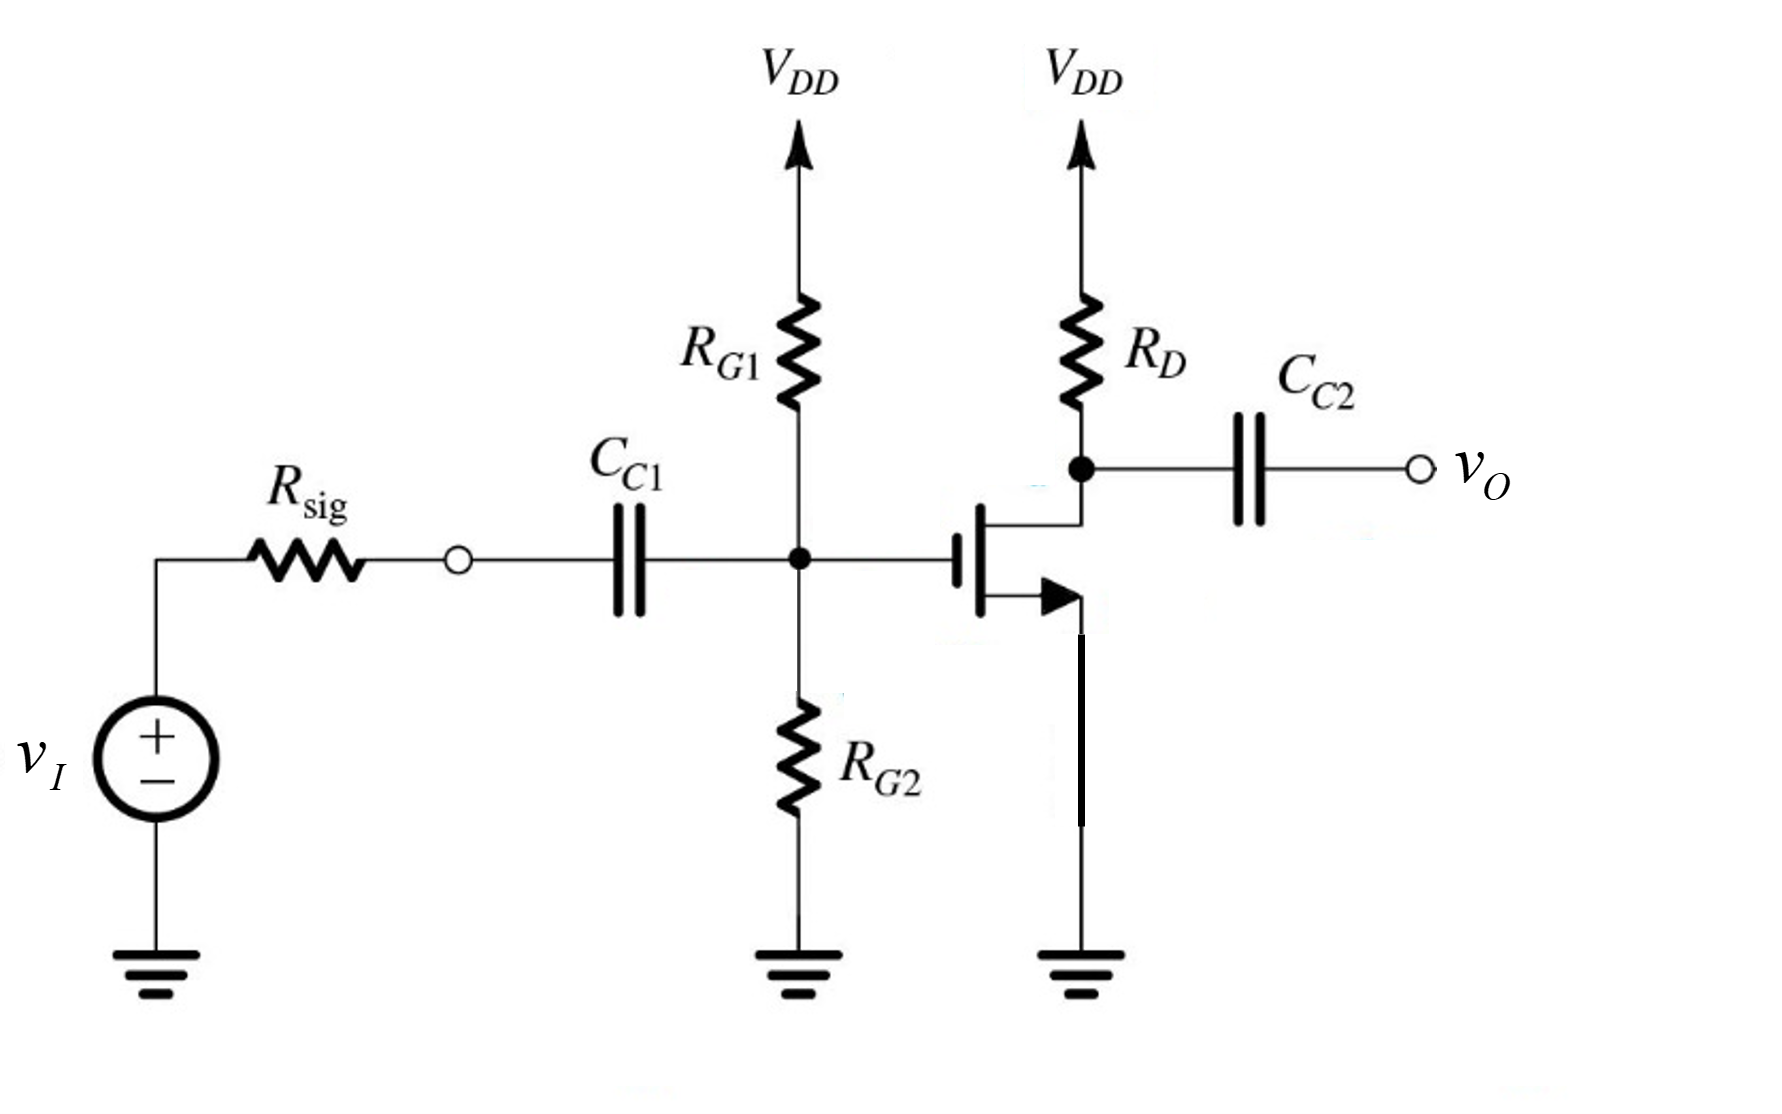
\includegraphics[width=4in]{schematic.png}
\end{center}

\begin{partquestion}{gainexpression}{The transistor is first biased such that $\frac{1}{4}V_{DD}$ drops across the resistor $R_{D}$. Give a simple expression for the small-signal voltage gain from gate to drain ($A_{v} = \frac{v_{d}}{v_{g}}$) only as a function of $V_{OV} = V_{GS} - V_{t}$. If $V_{OV} \geq 0.2\ \text{V}$, what is the maximum small-signal gain from gate to drain?}
\begin{answer}
Since one-fourth of the supply voltage $V_{DD}$ drops across the resistor $R_{D}$, we have:

\[
I_{D} = \frac{\frac{V_{DD}}{4}}{R_{D}} = \frac{2.5}{R_{D}}
\]

The common source gain with $\lambda = 0$ is:

\[
A_{v} = -g_{m}R_{D} = -\frac{2I_{D}}{V_{OV}}R_{D} = -\frac{2(2.5)}{V_{OV}R_{D}}R_{D} = -\frac{5}{V_{OV}}
\]

For $V_{OV} \geq 0.2$, we have:

\[
\left|A_{v}\right| \leq \frac{5}{0.2} = 25
\]
\end{answer}
\end{partquestion}

\begin{partquestion}{distortionlimit}{With $V_{OV} = 0.2\ \text{V}$, what is the limit to the ``small signal'' amplitude at the gate if we accept a second-order distortion term that is no more than 4\% of the first-order linear term (note this is stricter than the 10\% tolerance we discussed in class)?}
\begin{answer}
We saw from the lecture that the second-order (distortion) term is $\frac{1}{2}k v_{gs}^{2}$, and the first-order (linear) term is $g_{m}v_{gs} = kV_{OV}v_{gs}$. Comparing these two, if we want the second-order term to be less than 0.04 times the first-order term, we have:

\begin{align*}
    \frac{1}{2}k v_{gs}^2 &\leq 0.04 (k V_{OV} v_{gs}) \\
    v_{gs} &\leq 0.08 V_{OV} \\
    v_{gs} &\leq 0.08 (0.2) \\
    v_{gs} &\leq \qty{0.016}{\volt} \\
\end{align*}
\end{answer}
\end{partquestion}

\begin{partquestion}{currentchange}{With the small-signal limits in (b), what is the maximum \% change in $i_{D}$ (relative to $I_{D}$), to the nearest percent?}
\begin{answer}
This maximum change will occur when $i_{d}$ itself is at its maximum. We can calculate:

\begin{align*}
    \frac{i_{d\text{, max}}}{I_D} &= \frac{\left(\frac{2 I_D}{V_{OV}}\right)v_{gs} + \left(\frac{I_D}{V_{OV}^2}\right)v_{gs}^2}{I_D}\\
    &= 2\left(\frac{v_{gs}}{V_{OV}}\right) + \left(\frac{v_{gs}}{V_{OV}}\right)^2\\
    &= 2(0.08) + (0.08)^2\\
    &\approx 0.17
\end{align*}

Which is about 17\%! Amazing!
\end{answer}
\end{partquestion}

\begin{partquestion}{17dbgain}{Suppose the transistor or resistor is adjusted in an attempt to achieve $\left|A_{v}\right| = 17\ \text{dB}$ and the distortion constraints of part (b). Is this possible, and if so, find the largest small-signal amplitude that realizes this. Otherwise, what small-signal amplitude gets you closest to this gain? Assume $V_{OV}$ has the same constraint as in part (a).}
\begin{answer}
A gain of 17 dB is equivalent to a linear gain magnitude of $10^{\frac{17}{20}} = 7.08$. (Recall that the CS amplifier is an inverting amplifier, so we have a minus sign for the actual gain expression.) At this gain, we know from part (a) that

\[
V_{OV} = \frac{-5}{A_{v}} = \frac{-5}{-7.08} = 0.706\ \text{V}.
\]

This satisfies the constraint that $V_{OV} \geq 0.2\ \text{V}$, and $V_{DS} = \frac{3}{4}V_{DD} = 7.5\ \text{V} > V_{OV}$ so the device stays in saturation. It is clear that 17 dB of gain is achievable. Since from part (b) we know:

\begin{align*}
v_{gs} &\leq 2(0.04)V_{OV}\\
v_{gs} &\leq (0.08)(0.706\ \text{V})\\
v_{gs} &\leq 0.0565\ \text{V}.
\end{align*}

$v_{gs} = 0.0565\ \text{V}$ will achieve the desired gain.
\end{answer}
\end{partquestion}

\end{mainquestion}
